\chapter{WPAN Protocols}

\section{Bluetooth}
Bluetooth, known as 802.15, is a communication protocol designed in order to
create personal area networks (PAN). This opens up to new possibilities, such
as automatic synchronization of calendars between devices, or to transmission
of audio between smartphones and cars.

As you can see in Figure~\ref{fig:bt:btstack} the Bluetooth stack is modular.
You don't have to use all of it, you can use/implement only a subset. There are
different parts of the protocol:
\begin{itemize}
\item core protocol
\item cable replacement and telephony control protocol (RFCOMM and TCS BIN)
\item adopted protocol (use already existing protocols):
  \begin{AutoMultiColItemize}
  \item PPP
  \item TCP/UDP/IP
  \item OBEX
  \item WAE/WAP
  \end{AutoMultiColItemize}
\item radio
\item baseband
\item link manager protocol (LMP)
\item logical link control and adaptation protocol (L2CAP)
\item service discovery protocol (SDP)
\end{itemize}

\begin{figure}[t]
  \centering
  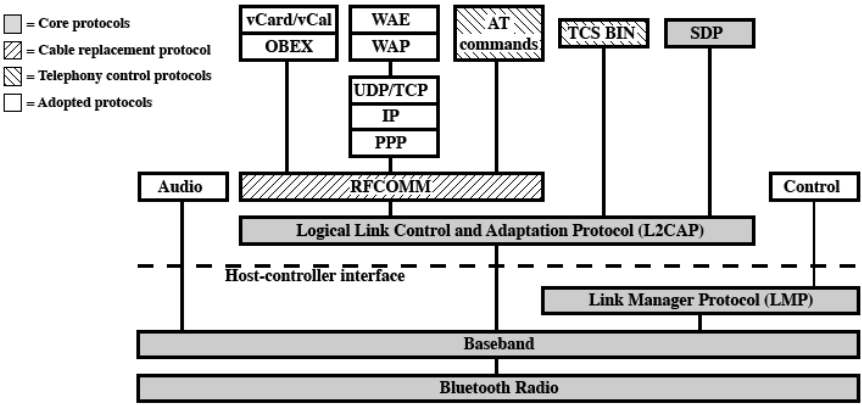
\includegraphics[scale=0.45]{BluetoothStack}
  \caption[Bluetooth stack]{A representation of the Bluetooth stack}
  \label{fig:bt:btstack}
\end{figure}

This modularity allows only some parts of the Bluetooth to be used, based on
the necessity. There are predefined configurations, called \textbf{profiles},
that are:
\begin{AutoMultiColItemize}
\item file transfer
\item internet bridge
\item LAN access
\item synchronization
\item three-in-one phone
\item headset
\end{AutoMultiColItemize}

\subsection{Bluetooth specifications}

Bluetooth topology can support up to seven simultaneous links in a logical star.
The peak data rate is of 1Mbps, using a band of 2.4GHz.
There is the capability to create a \textbf{piconet} or a \textbf{scatternet}.

\paragraph*{Piconet} A piconet is a collection of devices connected in an ad-hoc
fashion. One node will act as a master and the others as slaves for the duration
of the piconet connection: each master can connect up to 7 simultaneous devices
or 255 inactive slaves per piconet: all the slaves communicate through the
master, that doesn't polling to regulate communications, even the hopping
pattern.

\paragraph*{Scatternet} Piconets can be interconnected, with one master per
piconet, few devices are shared between the network, and it can be a combination
of Mater/Slave or Slave/Slave. This is still an ad-hoc network, without a
central structure. This mode allows many devices to share the same area, and
makes efficient use of bandwidth.

\paragraph*{Connection Setup} There are two scan typologies:
\textit{Inquiry-scan protocol} and \textit{Page-scan protocol}. The first one
learns about about the clock offset and device address of other nodes in
proximity, instead the second one establish links with nodes in proximity.

\section{ZigBee}

ZigBee is defined as 802.15.4 and its focus is mainly about power usage (over
100 times less energy required for connection operations). It uses mesh
networking, although it can use different topologies, as star and cluster tree.

\begin{figure}[t]
  \captionsetup{singlelinecheck=off}
  \centering
  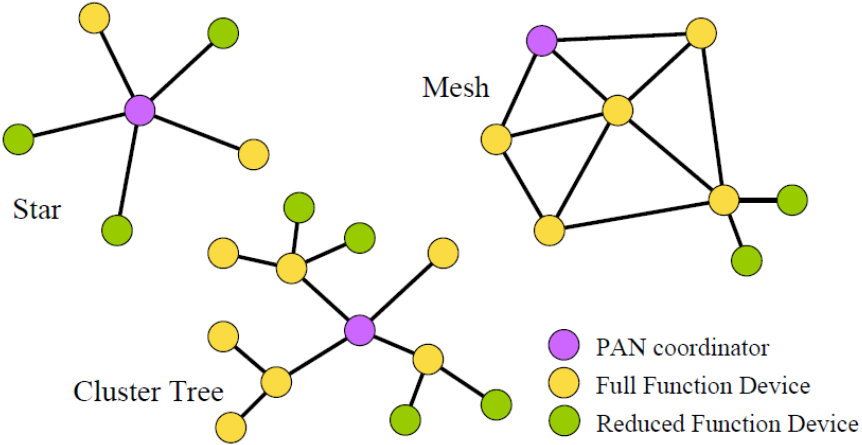
\includegraphics[scale=0.4]{ZigBeeTypology}
  \caption[ZigBee Topology]{
    ZigBee Typology. As you can see, there are different kind of devices:
    \begin{itemize}
    \item ZigBee coordinator (ZC): there is only one per network, it initiates
      the network formation and it may act as router once the network is formed
    \item ZigBee router (ZR): it's an optional network component, it may
      associate with a ZC or with another ZR and it can participate in multihop
      routing of messages
    \item ZigBee end device (ZED): it's an optional network component, that
      hasn't association and routing.
    \end{itemize}
  }
  \label{fig:zigbee:zbtopology}
\end{figure}

ZigBee supports up to 65k of nodes, and it's optimized for timing-critical
applications and power management. It only takes 15ms for a node to access the
channel, and 30ms to join the network.
With WiFi you need seconds to perform this actions. These sorts times make the
system very reactive.

\paragraph*{Wibree} Wibree is a Bluetooth version that tries to reach ZigBee
low-energy and performance. It hasn't Bluetooth frequency hopping and uses the
same Bluetooth hardware.

\subsection{ZigBee vs Bluetooth}

There are main differences with Bluetooth. BT is designed to be a cable
replacement for this sort of things:
\begin{itemize}
\item synchronization of call phone to PDA
\item hands-free audio
\end{itemize}
ZigBee instead works better where there are:
\begin{AutoMultiColItemize}
\item Controls
\item Sensors
\item Small data packets
\item Long battery is critical
\end{AutoMultiColItemize}
ZigBee is more suited for medic transfer or data transfer.
